\section{Modeling and systematic uncertainties}
\lb{sec:lowE_syst}

In this appendix we study the dependence of the spectrum of gamma-ray emission at the base of the FB
on the selection of the low energy range in the definition of the diffuse foreground model
and on the choice of the class of the events (ultraclean vs source).
We use the rectangles model of the FB in Section \ref{sec:box_model}
as our baseline example.
In this model, the foreground emission model template consists of Source-class data averaged over the energy interval $0.3 - \SI{1.0}{GeV}$. 
To probe the dependence on the choice of the low-energy range in the baseline model, 
we pick three non-overlapping energy ranges $0.3 - \SI{0.5}{GeV}$, $0.5 - \SI{1.0}{GeV}$, and $1.0 - \SI{2.2}{GeV}$ 
and use the same analysis as for the baseline model. 
We also compare with the spectra obtained using Ultraclean class data both in the definition of the model
at low energies and in the analysis at high energies.
The residual spectra resulting from the different energy ranges and data classes are shown in Figure \ref{fig:syst_models}. 
The agreement among the models is relatively good at $E > 10$ GeV, especially for negative longitudes.

\begin{figure*}[h]
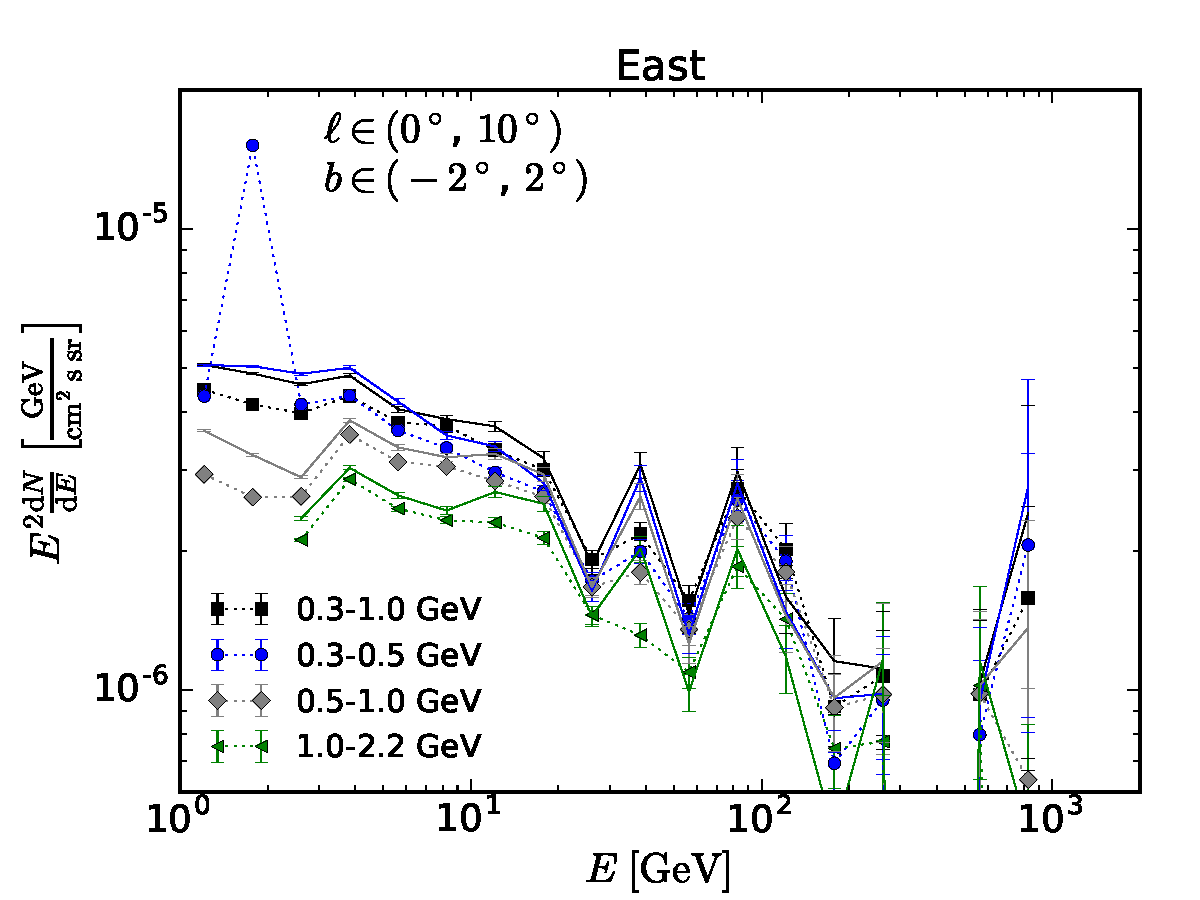
\includegraphics[width=0.5\textwidth]{plots/SED_different_lowE_ranges_boxes_l=5_b=0.pdf}
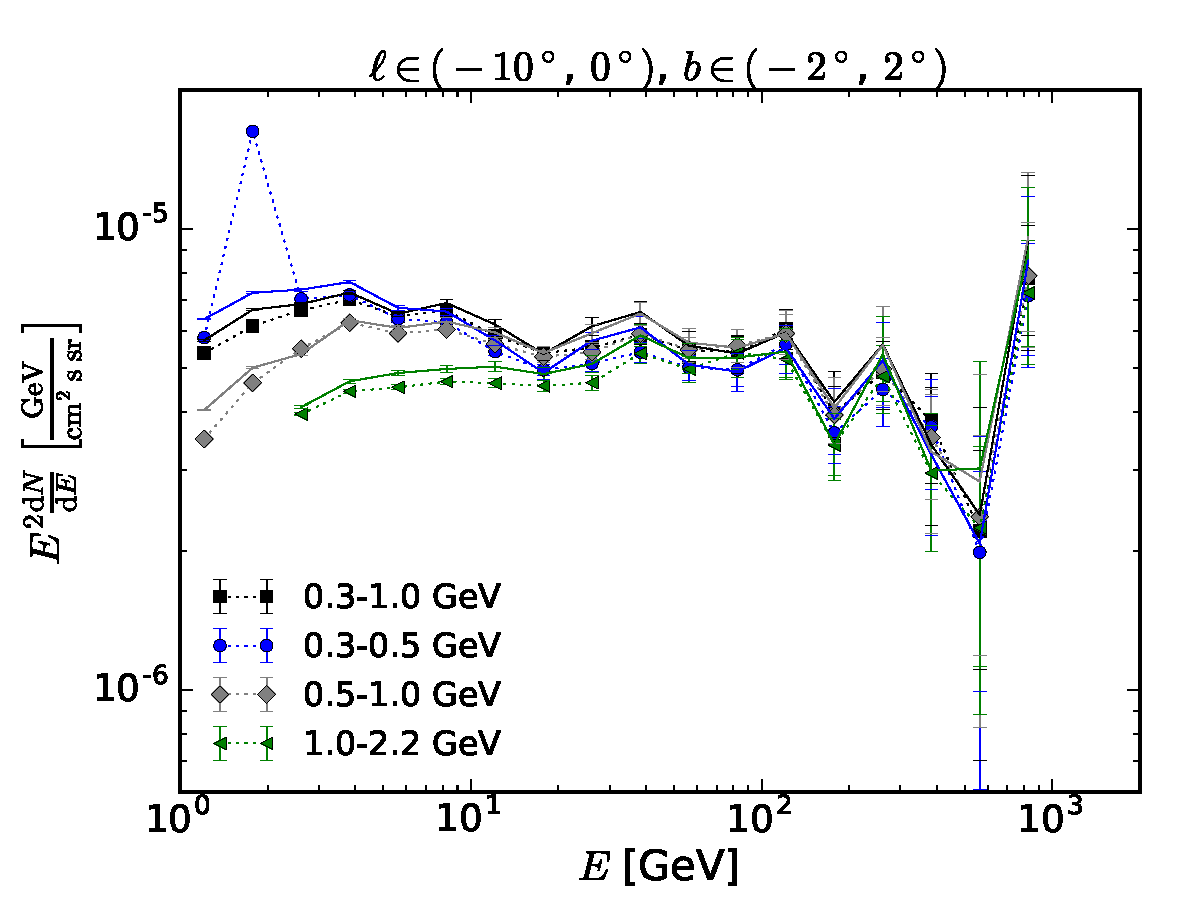
\includegraphics[width=0.5\textwidth]{plots/SED_different_lowE_ranges_boxes_l=-5_b=0.pdf}
\caption{SED of the residual in the rectangles model using Source class (dotted lines with markers) and Ultraclean class data (solid lines) in four different energy ranges. The baseline model, presented in Section \ref{sec:box_model}, has the low-energy range in the definition of the foreground model
$0.3 - \SI{1.0}{GeV}$ (black squres).}
\label{fig:syst_models}
\end{figure*}